% PRIOR POSTERIOR COUPLING
Given the prior distribution and the likelihood function, Bayes' rule characterizes the posterior as a conditional density.
It is interesting to view the transition from the prior to the posterior density in terms of random variables instead.
While that point of view is not directly suggested by Bayes's law, which only operates on probability densities,
it indeed provides some useful intuition and leads to new recipes for computational Bayesian inference.
This is investigated next.
\par % PRIOR TRANSFORMATION
Consider an injective and continuously differentiable map \(\map \colon \mathds{R}^{\dimParam} \rightarrow \mathds{R}^{\dimParam}\) that transforms a random variable
\(\bm{X} \sim \pi(\bm{x})\) distributed according to the prior distribution into a new random variable
\begin{equation} \label{eq:Transport:PosteriorRV}
  \tilde{\bm{X}} = \map(\bm{X}) \sim \pi_{\map}(\tilde{\bm{x}}).
\end{equation}
The map is assumed to be invertible and sufficiently well-behaved, such that one can write the transformed density of the random variable in \cref{eq:Transport:PosteriorRV} as
\begin{equation} \label{eq:Transport:PriorTransformation}
  \pi_{\map}(\tilde{\bm{x}})
  = \pi(\map^{-1}(\tilde{\bm{x}})) \, \lvert \det J_{\map^{-1}}(\tilde{\bm{x}}) \rvert.
\end{equation}
% POSTERIOR TRANSFORMATION
Conversely, given that a random variable \(\tilde{\bm{X}} \sim \pi(\tilde{\bm{x}} \cond \bm{y})\) is distributed according to the posterior,
one may consider the back-transformation \(\bm{X} = \map^{-1}(\tilde{\bm{X}}) \sim \pi_{\map^{-1}}(\bm{x} \cond \bm{y})\) with
\begin{equation} \label{eq:Transport:PosteriorBacktransformation}
  \pi_{\map^{-1}}(\bm{x} \cond \bm{y})
  = \pi(\map(\bm{x}) \cond \bm{y}) \, \lvert \det J_\map(\bm{x}) \rvert
  = \frac{\mathcal{L}(\map(\bm{x})) \pi(\map(\bm{x}))}{\scale} \, \lvert \det J_\map(\bm{x}) \rvert.
\end{equation}
% DETERMINISTIC COUPLING
One is interested in such maps \(\map\) for which the transformed prior \(\pi_{\map}\) in \cref{eq:Transport:PriorTransformation} equals the posterior
and the back-transformed posterior \(\pi_{\map^{-1}}(\cdot \cond \bm{y})\) in \cref{eq:Transport:PosteriorBacktransformation} equates to the prior.
This means that
\begin{equation} \label{eq:Transport:PriorPosteriorTransformation}
  \pi_{\map} = \pi(\cdot \cond \bm{y}), \quad \pi_{\map^{-1}}(\cdot \cond \bm{y}) = \pi.
\end{equation}
In this sense, the prior and the posterior density transform into one another.
Given the prior random vector \(\bm{X} \sim \pi(\bm{x})\), the transformed random vector \(\tilde{\bm{X}} \sim \pi(\tilde{\bm{x}} \cond \bm{y})\) follows the posterior.
While \cref{eq:Transport:PriorPosteriorTransformation} is formulated in terms of densities, it also establishes a \emph{deterministic coupling}
\((\bm{X},\map(\bm{X}))\) of the prior and the posterior probability measure \cite{Probability:Thorisson2000,Probability:Lindvall2002}.
\par % ILLUSTRATION
An illustration of this principle is given in \cref{fig:Transport:PriorTransformation}, where both the prior and the posterior are Gaussian distributions.
This is the same setup as already visualized in \cref{fig:Bayesian:BayesianInference}.
Two linear transformations are shown that transform the prior into the posterior density.
For more complex problems involving non-Gaussian distributions the transformations will be generally nonlinear, though.
% FIGURE: PRIOR TRANSFORMATION
\begin{figure}[htbp]
  \centering
  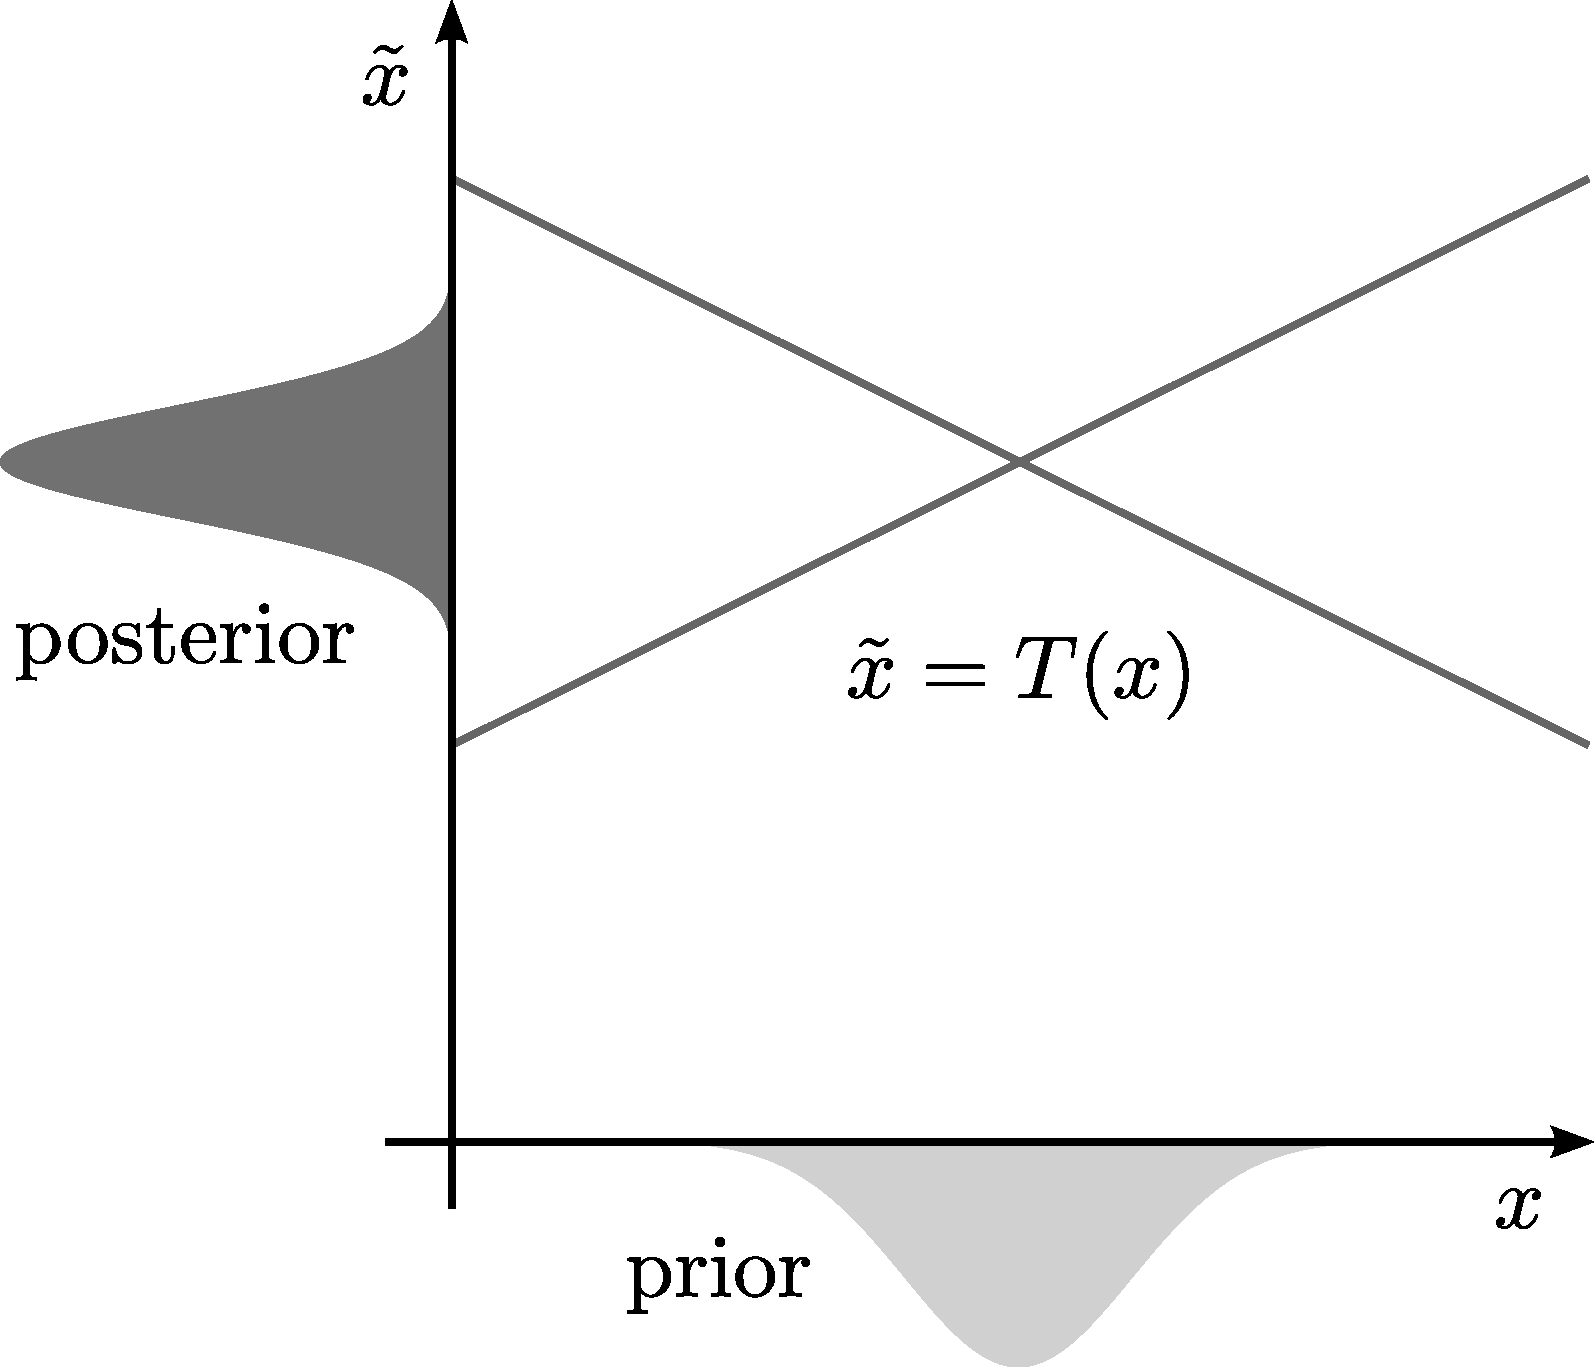
\includegraphics[width=7cm]{fig_Transport_PriorTransformation}
  \caption[Prior transformation]{Prior transformation.}
  \label{fig:Transport:PriorTransformation}
\end{figure}

\subsection{Couplings of Gaussians}
% GAUSSIAN RANDOM VARIABLES
Motivated by the illustrative example above, we study the case involving Gaussian distributions in greater depth.
Consider two real-valued Gaussian random variables \(X_1 \sim \mathcal{N}(x_1 \cond \mu_1, \sigma_1^2)\) and \(X_2 \sim \mathcal{N}(x_2 \cond \mu_2, \sigma_2^2)\).
Their respective distributions have means \(\mu_1\) and \(\mu_2\) and variances \(\sigma_1^2\) and \(\sigma_2^2\).
% DETERMINISTIC COUPLING
The first distribution transforms into the second one by
\begin{equation} \label{eq:Transport:UnivariateGaussianTransformation}
  x_2 = \map(x_1) = \mu_2 \pm \frac{\sigma_2}{\sigma_1}(x_1 - \mu_1)
\end{equation}
Two different linear couplings between the Gaussian distributions are described by \cref{eq:Transport:UnivariateGaussianTransformation}
for which the variance transforms as \(\sigma_2^2 = \sigma_1^2 (\pm \sigma_2 / \sigma_1)^2\).
In the case that the random variables \(X_1 \sim \mathcal{N}(x_1 \cond \mu_1, \sigma_1^2) = \pi(x_1)\) and \(X_2 \sim \mathcal{N}(x_2 \cond \mu_2, \sigma_2^2) = \pi(x_2 \cond \bm{y})\)
are distributed according to the prior and the posterior of Gaussian shape, respectively, this is exactly the scenario encountered in \cref{fig:Transport:PriorTransformation}.
\par % GAUSSIAN RANDOM VECTORS
Now consider two \(\mathds{R}^\dimParam\)-valued random variables \(\bm{X}_1 \sim \mathcal{N}(\bm{x}_1 \cond \bm{\mu}_1,\bm{\Sigma}_1)\)
and \(\bm{X}_2 \sim \mathcal{N}(\bm{x}_2 \cond \bm{\mu}_2,\bm{\Sigma}_2)\).
They have Gaussian distributions with mean vectors \(\bm{\mu}_1\) and \(\bm{\mu}_2\) and covariance matrices \(\bm{\Sigma}_1\) and \(\bm{\Sigma}_2\), respectively.
% MATRIX SQUARE ROOT
Let \(\bm{\Sigma}^{1/2}\) denote the principle square root of a symmetric and positive-definite matrix \(\bm{\Sigma}\)
that is uniquely characterized by \(\bm{\Sigma} = \bm{\Sigma}^{1/2} \bm{\Sigma}^{1/2}\).
% DETERMINISTIC COUPLING
In a straightforward manner, a deterministic coupling between the multivariate normal distributions is established by
\begin{equation} \label{eq:Transport:StandardGaussianCoupling}
  \bm{x}_2 = \map(\bm{x}_1) = \bm{\mu}_2 + \bm{\Sigma}_2^{1/2} \bm{\Sigma}_1^{-1/2}(\bm{x}_1 - \bm{\mu}_1).
\end{equation}
Indeed one has \(\bm{\Sigma}_2 = (\bm{\Sigma}_2^{1/2} \bm{\Sigma}_1^{-1/2}) \bm{\Sigma}_1 (\bm{\Sigma}_2^{1/2} \bm{\Sigma}_1^{-1/2})^\top\).
More generally, \(\bm{\Sigma}_2 = (\bm{\Sigma}_2^{1/2} \bm{\Phi} \bm{\Sigma}_1^{-1/2}) \bm{\Sigma}_1 (\bm{\Sigma}_2^{1/2} \bm{\Phi} \bm{\Sigma}_1^{-1/2})^\top\)
for an arbitrary orthogonal matrix \(\bm{\Phi}\) with \(\bm{\Phi}^\top \bm{\Phi} = \bm{\Phi} \bm{\Phi}^\top = \bm{I}\).
% NON-UNIQUENESS
Hence, the coupling in \cref{eq:Transport:StandardGaussianCoupling} is non-unique since any such \(\bm{\Phi}\) defines an appropriate coupling by
\begin{equation} \label{eq:Transport:ArbitraryGaussianCoupling}
  \bm{x}_2 = \map(\bm{x}_1) = \bm{\mu}_2 + \bm{\Sigma}_2^{1/2} \bm{\Phi} \bm{\Sigma}_1^{-1/2}(\bm{x}_1 - \bm{\mu}_1).
\end{equation}
\par % DISCUSSION
The just-mentioned transforms define well-behaved couplings between Gaussian distributions that exhibit Jacobian formulas for the change of variables.
More generally, non-continuous transformations may accomplish the same purpose, e.g.\ piecewise combinations of the linear transformations discussed, but cannot be written that nicely.
In the following we exclusively concentrate on invertible and continuously differentiable maps.
Beforehand, some introductory remarks on optimal transportation are given.
This framework gives rise to important statements regarding the existence and uniqueness of deterministic couplings between general probability distributions, not only Gaussians.

\subsection{Optimal transportation}
% OPTIMAL TRANSPORTATION
As the preceding discussion revealed, a suitable map that transforms the prior into the posterior may not be unique.
It may not even exist in the general case.
In the framework of \emph{optimal transport theory} \cite{Transport:Villani2003,Transport:Villani2008}, however, one can establish certain existence and uniqueness results.
A map \(\map\) that satisfies \(\pi_{\map} = \pi(\cdot \cond \bm{y})\) is called a \emph{transport map} in this context.
% COST FUNCTION
Let a cost function \(c \colon \mathds{R}^{\dimParam} \times \mathds{R}^{\dimParam} \rightarrow \mathds{R}^{+}\)
represent the expense \(c(\bm{x},\tilde{\bm{x}})\) of transporting a unit mass from \(\bm{x}\) to \(\tilde{\bm{x}}\).
The total cost of the mapping \(\tilde{\bm{x}} = \map(\bm{x})\) is then
\begin{equation} \label{eq:Transport:TotalCost}
  C(\map) = \int\limits_{\mathds{R}^{\dimParam}} c(\bm{x}, \map(\bm{x})) \, \pi(\bm{x}) \, \mathrm{d} \bm{x}.
\end{equation}
% MONGE PROBLEM
The \emph{Monge problem} asks for finding a transport map that is optimal in that it minimizes the transportation cost in \cref{eq:Transport:TotalCost}.
As expressed in our density-oriented language and notation, this means to
\begin{equation} \label{eq:Transport:MongeProblem}
  \begin{aligned}
    & \text{minimize} & & C(\map), \\
    & \text{subject to} & & \pi_{\map} = \pi(\cdot \cond \bm{y}).
  \end{aligned}
\end{equation}
\par % BRENIER-McCANN
A solution to the problem in \cref{eq:Transport:MongeProblem} is called an \emph{optimal transport map}.
Under relatively weak assumptions regarding the distributions involved and the cost function, one can ensure the existence and uniqueness of such an optimal map,
e.g.\ for a quadratic cost function \(c(\bm{x},\tilde{\bm{x}}) = \lVert \bm{x} - \tilde{\bm{x}} \rVert_2^2\)
such results are established by the \emph{Brenier--McCann theorem} \cite{Transport:Brenier1991,Transport:McCann1995}.
Moreover, it states that the map is monotone.
% KNOTHE-ROSENBLATT
Under certain other cost considerations, the optimal map can be shown to coincide with the \emph{Knothe--Rosenblatt rearrangement} \cite{Transport:Carlier2010,Transport:Bonnotte2013}.
This means that the transport map has a triangular structure.
\par % MONGE-KANTOROVICH PROBLEM
For the sake of completeness, it is remarked that the \emph{Monge--Kantorovich problem} is a generalization of the problem discussed above.
It allows for transport plans \(\pi(\bm{x},\tilde{\bm{x}})\) and more general couplings \((\bm{X},\tilde{\bm{X}})\)
that admit the marginals \(\bm{X} \sim \pi(\bm{x})\) and \(\tilde{\bm{X}} \sim \pi(\tilde{\bm{x}} \cond \bm{y})\).
The trivial coupling with \(\pi(\bm{x},\tilde{\bm{x}}) = \pi(\bm{x}) \pi(\tilde{\bm{x}} \cond \bm{y})\)
and the deterministic coupling with \(\tilde{\bm{X}} = \map(\bm{X})\) discussed above are two extreme cases.
An optimal transference plan minimizes the total cost
\(C(\map) = \iint_{\mathds{R}^{\dimParam} \times \mathds{R}^{\dimParam}} c(\bm{x},\tilde{\bm{x}}) \, \pi(\bm{x},\tilde{\bm{x}}) \, \mathrm{d} \bm{x} \, \mathrm{d} \tilde{\bm{x}}\).
Non-deterministic couplings are not permitted in Monge's original problem formulation which we actually focus on.
However, for future research endeavors it may be useful to keep this possibility in mind.
\par % REGULARIZATION
In the Bayesian context, one is only interested in the transformation properties of the map and may thus safely disregard its cost and optimality.
Indeed, here the map is merely an auxiliary construct with no associated transportation cost whatsoever.
Hence, any arbitrary transport map is as good as any other.
Yet, imposing an auxiliary cost function may still guide the practical computation of a transport map with a convenient structure, i.e.\ it regularizes the problem.
Note that the quadratic cost function would favor maps close to the identity.
This would for example suggest to pick the monotonically increasing transport map and scrap the decreasing one
in \cref{fig:Transport:PriorTransformation} or \cref{eq:Transport:UnivariateGaussianTransformation}.
Other cost functions would promote other structures, e.g.\ triangular maps.